\begin{name}
	{\tenchude}{ĐỀ ÔN TẬP SỐ 4}{LỚP TOÁN THẦY PHÁT}{\thoigian}
\end{name}
\setcounter{ex}{0}
\setcounter{bt}{0}
\Opensolutionfile{ans}[ans/ans-Vted-14-2023]
%%==========Câu 1
\begin{ex}%[Dự án 12-Vted-2022, Quan Ón]%[1D2Y2-1]
		Với $n$, $k$ là các số nguyên dương và $k \leq n$, công thức nào dưới đây đúng?
		\choice
		{$\mathrm{C}^k_n = n!\mathrm{A}^k_n$}
		{$\mathrm{C}^k_n = k!\mathrm{A}^k_n$}
		{$\mathrm{C}^k_n = \dfrac{\mathrm{A}^k_n}{n!}$}
		{\True $\mathrm{C}^k_n = \dfrac{\mathrm{A}^k_n}{k!}$}
	\loigiai{
		Ta có $\mathrm{C}^k_n = \dfrac{\mathrm{A}^k_n}{k!}$.
	}
\end{ex}

%%==========Câu 2
\begin{ex}%[Dự án 12-Vted-2022, Quan Ón]%[2H3Y2-4]
	Trong KG $Oxyz$, đường thẳng $d\colon \dfrac{x-1}{2} = \dfrac{y+2}{-1} = \dfrac{z + 3}{3}$ đi qua điểm nào dưới đây?
	\choice
	{$M(2;-1;3)$}
	{$P(-2;1;-3)$}
	{\True $Q(1;-2;-3)$}
	{$N(-1;2;3)$}
	\loigiai{
		Đường thẳng $d\colon \dfrac{x-1}{2} = \dfrac{y+2}{-1} = \dfrac{z + 3}{3}$ đi qua điểm $Q(1;-2;-3)$.
	}
\end{ex}

%%==========Câu 3
\begin{ex}%[Dự án 12-Vted-2022, Quan Ón]%[2H1Y3-2] 
	Thể tích của khối lập phương cạnh bằng $6$ là
	\choice
	{$108$}
	{\True $216$}
	{$6$}
	{$36$}
	\loigiai{
		Thể tích của khối lập phương cạnh bằng $6$ là $V = 6^3 = 216$.
	}
\end{ex}

%%==========Câu 4
\begin{ex}%[Dự án 12-Vted-2022, Quan Ón]%[2D2Y5-2]
	Nghiệm của phương trình $\log_{2}(x-4) = 3$ là
	\choice
	{$x = 8$}
	{$x = 13$}
	{$x = 10$}
	{\True $x = 12$}
	\loigiai{
		Điều kiện xác định $x - 4 > 0 \Leftrightarrow x > 4$.\\
		Ta có
		$$ \log_{2}(x-4) = 3 \Leftrightarrow x - 4 = 2^3 \Leftrightarrow x - 4 = 8 \Leftrightarrow x = 12 \textrm{ (nhận).} $$
	}
\end{ex}

%%==========Câu 5
\begin{ex}%[Dự án 12-Vted-2022, Quan Ón]%[2D3Y2-1]
	Nếu $\displaystyle \int\limits_{2}^{5}f(x)dx = 2$ thì với số thực $k$ tùy ý, $\displaystyle \int\limits_{2}^{5}k\cdot f(x)dx$ bằng
	\choice
	{\True $2k$}
	{$-6k$}
	{$6k$}
	{$-2k$}
	\loigiai{
		Ta có $\displaystyle \int\limits_{2}^{5}k\cdot f(x)dx = k\cdot \displaystyle \int\limits_{2}^{5}f(x)dx = k\cdot 2 = 2k$.
	}
\end{ex}

%%==========Câu 6
\begin{ex}%[Dự án 12-Vted-2022, Quan Ón]%[2D1Y5-4]
	Điểm nào dưới đây thuộc đồ thị của hàm số $y = \dfrac{2x - 1}{x + 2}$?
	\choice
	{\True $M\left( 1;\dfrac{1}{3} \right)$}
	{$Q(-1;3)$}
	{$P(1;1)$}
	{$N(-1;-2)$}
	\loigiai{
		Thay $x = 1$ vào $y = \dfrac{2x - 1}{x + 2}$ ta được $y = \dfrac{2x - 1}{x + 2} = \dfrac{2\cdot 1 - 1}{1 + 2} = \dfrac{1}{3}$.\\
		Do đó điểm $M\left( 1;\dfrac{1}{3} \right)$ thuộc đồ thị của hàm số $y = \dfrac{2x - 1}{x + 2}$.
	}
\end{ex}

%%==========Câu 7
\begin{ex}%[Dự án 12-Vted-2022, Quan Ón]%[2D2Y6-2] 
	Tập nghiệm của bất phương trình $2^x < 6$ là
	\choice
	{$(\log_{2}6; +\infty)$}
	{$(-\infty; 3)$}
	{$(3; + \infty)$}
	{\True $(-\infty; \log_{2}6)$}
	\loigiai{
		Ta có $2^x < 6 \Leftrightarrow x < \log_{2}6$.\\
		Do đó, tập nghiệm của bất phương trình $2^x < 6$ là $(-\infty; \log_{2}6)$.
	}
\end{ex}

%%==========Câu 8
\begin{ex}%[Dự án 12-Vted-2022, Quan Ón]%[1D3Y4-3] 
	Cho cấp số nhân $(u_n)$ với $u_1 = 7$ và công bội $q = 4$. Giá trị của $u_2$ bằng
	\choice
	{$11$}
	{$3$}
	{$\dfrac{7}{4}$}
	{\True $28$}
	\loigiai{
		Vì cấp số nhân $(u_n)$ có $u_1 = 7$ và công bội $q = 4$ nên $u_2 = u_1q = 7\cdot 4 = 28$.\\
		Vậy $u_2 = 28$.
	}
\end{ex}

%%==========Câu 9
\begin{ex}%[Dự án 12-Vted-2022, Quan Ón]%[2H3Y1-3]
	Trong KG $Oxyz$, mặt cầu $(S)\colon (x-2)^2 + (y+8)^2 + z^2 = 9$ có tâm là điểm nào dưới đây?
	\choice
	{$M(-1;4;0)$}
	{$N(1;-4;0)$}
	{$P(-2;8;0)$}
	{\True $Q(2;-8;0)$}
	\loigiai{
		Mặt cầu $(S)\colon (x-2)^2 + (y+8)^2 + z^2 = 9$ có tâm là điểm $Q(2;-8;0)$.
	}
\end{ex}

%%==========Câu 10
\begin{ex}%[Dự án 12-Vted-2022, Quan Ón]%[2D2Y4-1]
Tập xác định của hàm số $y = x^{\tfrac{3}{2}}$ là
	\choice
	{\True $(0;+\infty)$}
	{$\mathbb{R}$}
	{$\mathbb{R}\setminus \left\lbrace 0 \right\rbrace $}
	{$[0;+\infty)$}
\loigiai{
Vì $\dfrac{3}{2} \notin \mathbb{Z}$ nên tập xác định của hàm số $y = x^{\tfrac{3}{2}}$ là $\mathcal{D} = (0;+\infty)$.
}
\end{ex}



%%==========Câu 11
\begin{ex}%[Dự án 12-Vted-2022, Thien Tran Xuan]%[2D4B2-2]
Trên mặt phẳng tọa độ, cho $M(2; 3)$ là điểm biểu diễn của số phức $z$. Phần ảo của $z$ bằng
\choice
{$2$}
{\True $3$}
{$-3$}
{$-2$}
\loigiai{Phần ảo của $z$ bằng $3$.
}
\end{ex}

%%==========Câu 12
\begin{ex}%[Dự án 12-Vted-2022, Thien Tran Xuan]%[2D1Y5-1]
\immini{Hàm số nào dưới đây có đồ thị như đường cong trong hình bên?
	\choice
	{$y = -x^3 + 3x - 1$}
	{$y = \dfrac{x + 1}{x - 1}$}
	{\True $y = x^3 - 3x - 1$}
	{$y = x^4 - 2x^2 - 1$}
	}{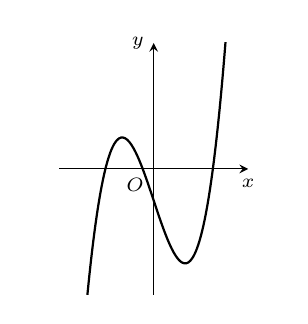
\begin{tikzpicture}[>=stealth,x=1cm,y=1cm,scale=0.4]
		\def\a{1} % Hệ số a phải khác 0
		\def\b{0}
		\def\c{-3}
		\def\d{-1}
		\draw[->] (-3,0) -- (3,0)node[below]{\scriptsize $x$};
		\draw[->] (0,-4) -- (0,4) node[left] {\scriptsize $y$};
		\draw (0,0)node[below left]{\scriptsize $O$};
		\clip (-4,-4)rectangle(4,4);
		\draw[thick,samples=150,smooth,domain=-5:5] plot(\x,{\a*(\x)^3+(\b)*(\x)^2+(\c)*\x+(\d)});
	\end{tikzpicture}
	}
\loigiai{
Hàm số đã cho là đồ thị hàm số bậc ba với hệ số $a > 0$ nên đồ thị đã cho là đồ thị hàm số $y = x^3 - 3x - 1$.
}
\end{ex}

%%==========Câu 13
\begin{ex}%[Dự án 12-Vted-2022, Thien Tran Xuan]%[2H1Y3-2]
Cho khối chóp có diện tích đáy $B = 5a^2$ và chiều cao $h = a$. Thể tích của khối chóp đã cho bằng
\choice
{\True $\dfrac{5}{6}a^3$}
{$\dfrac{5}{2}a^3$}
{$5a^3$}
{$\dfrac{5}{3}a^3$}
\loigiai{
Thể tích của khối chóp đã cho là $V = \dfrac{1}{3}Bh = \dfrac{1}{3} \cdot 5a^2 \cdot a = \dfrac{5}{3}a^3$ (đvtt).
}
\end{ex}

%%==========Câu 14
\begin{ex}%[Dự án 12-Vted-2022, Thien Tran Xuan]%[2H3Y2-2]
Trong KG $Oxyz$, cho mặt phẳng $(P) \colon 3x - y + 2z - 1 = 0$. Véctơ nào dưới đây là một véctơ pháp tuyến của $(P)$ ?
\choice
{$\vec{n}_1 = (-3; 1; 2)$}
{\True $\overrightarrow{n}_2 = (3; -1; 2)$}
{$\overrightarrow{n}_3 = (3; 1; 2)$}
{$\overrightarrow{n}_4 = (3; 1; -2)$}
\loigiai{
Véctơ $\overrightarrow{n}_2 = (3; -1; 2)$ là một véctơ pháp tuyến của $(P)$.
}
\end{ex}

%%==========Câu 15
\begin{ex}%[Dự án 12-Vted-2022, Thien Tran Xuan]%[2D4B2-2]
Cho số phức $z = 3 - 2i$, khi đó $2 \cdot \overline{z}$ bằng
\choice
{$-6 - 4i$}
{$6 - 4i$}
{\True $6 + 4i$}
{$-6 + 4i$}
\loigiai{
Ta có $\overline{z} = 3 + 2i$. Suy ra $2 \cdot \overline{z} = 6 + 4i$.
}
\end{ex}

%%==========Câu 16
\begin{ex}%[Dự án 12-Vted-2022, Thien Tran Xuan]%[2H2Y1-2]
Cho hình nón có bán kính đáy $r$ và độ dài đường sinh $\ell$. Diện tích xung quanh $S_{xq}$ của hình nón đã cho được tính theo công thức nào dưới đây?
\choice
{$S_{xq} = \pi r(r + \ell)$}
{$S_{xq} = 2 \pi r\ell$}
{$S_{xq} = 2 \pi r(r +\ell)$}
{\True $S_{xq} = \pi r\ell$}
\loigiai{
Diện tích xung quanh $S_{xq}$ của hình nón đã cho được tính theo công thức $S_{xq} = \pi r\ell$.
}
\end{ex}

%%==========Câu 17
\begin{ex}%[Dự án 12-Vted-2022, Thien Tran Xuan]%[2D4B2-2]
Phần thực của số phức $z = 5 - 2i$ bằng
\choice
{\True $5$}
{$2$}
{$-5$}
{$-2$}
\loigiai{
Phần thực của số phức $z = 5 - 2i$ bằng $5$.
}
\end{ex}

%%==========Câu 18
\begin{ex}%[Dự án 12-Vted-2022, Thien Tran Xuan]%[2H2B2-1]
Trong KG $Oxyz$, cho đường thẳng $d$ đi qua điểm $M(3; -1; 4)$ và có một véc-tơ chỉ phương $\vec{u} = (-2; 4; 5)$. Phương trình của $d$ là
\choice
{$\heva{&x = -2 + 3t\\&y = 4 - t\\&z = 5 + 4t}$}
{$\heva{&x = 3 + 2t\\&y = -1 + 4t\\&z = 4 + 5t}$}
{$\heva{&x = 3 - 2t\\&y = 1 + 4t\\&z = 4 + 5t}$}
{\True $\heva{&x = 3 - 2t\\&y = -1 + 4t\\&z = 4 + 5t}$}
\loigiai{
Phương trình của $d$ là $\heva{&x = 3 - 2t\\&y = -1 + 4t\\&z = 4 + 5t}$.
}
\end{ex}

%%==========Câu 19
\begin{ex}%[Dự án 12-Vted-2022, Thien Tran Xuan]%[2D1Y4-1]
Tiệm cận đứng của đồ thị hàm số $y = \dfrac{2x - 1}{x - 1}$ là đường thẳng có phương trình
\choice
{\True $x = 1$}
{$x = -1$}
{$x = 2$}
{$x = \dfrac{1}{2}$}
\loigiai{
Tiệm cận đứng của đồ thị hàm số $y = \dfrac{2x - 1}{x - 1}$ là đường thẳng có phương trình $x = 1$.
}
\end{ex}

%%==========Câu 20
\begin{ex}%[Dự án 12-Vted-2022, Thien Tran Xuan]%[2D3B2-1]
Nếu $\displaystyle\int\limits_1^4 f(x) \mathrm{\,d} x=3$ và $\displaystyle\int\limits_1^4 g(x) \mathrm{\,d}x = -2$ thì $\displaystyle\int\limits_1^4[f(x)-g(x)] \mathrm{\,d}x$ bằng
\choice
{$-1$}
{$-5$}
{\True $5$}
{$1$}
\loigiai{
Ta có $\displaystyle\int\limits_1^4[f(x)-g(x)] \mathrm{\,d}x = \displaystyle\int\limits_1^4 f(x) \mathrm{\,d}x - \displaystyle\int\limits_1^4 g(x) \mathrm{\,d}x = 3 - (-2) = 5$.
}
\end{ex}

%%==========Câu 21
\begin{ex}%[Dự án 12-Vted-2022, Tin Dat Tran]%[2D2Y4-2]
Trên khoảng $(0 ;+\infty)$, đạo hàm của hàm số $y=\log (2 x)$ là
\choice
{$y'=\dfrac{1}{2 x \ln 2}$}
{$y'=\dfrac{1}{2 x \ln 10}$}
{\True $y'=\dfrac{1}{x \ln 2}$}
{$y'=\dfrac{1}{x \ln 10}$}
\loigiai{
	Trên khoảng $(0 ;+\infty)$, ta có $y'=\dfrac{1}{2x\ln 2}\cdot (2x)'=\dfrac{1}{x\ln 2}$.
}
\end{ex}

%%==========Câu 22
\begin{ex}%[Dự án 12-Vted-2022, Tin Dat Tran]%[2D1Y2-2]
Cho hàm số $y=f(x)$ có bảng biến thiên như sau:
\begin{center}
	
\begin{tikzpicture}[font=\normalsize,t style/.style={style=solid}]
		%dòng khai báo
		\tkzTabInit[nocadre=true,lgt=1.2,espcl=2.5,deltacl=0.5]
		{$x$ /0.65, $y'$/0.65, $y$/2}
		{$ -\infty $,$ -1 $,$ 1 $,$ +\infty $}
		%dòng xét dấu
		\tkzTabLine{  , -,0 , +, 0 , -,  }  % z, t, d;
		%dòng biến thiên
		\tkzTabVar{+/$-\infty$,-/$-3$,+/$5$,-/$-\infty$} %+ hoac-
	\end{tikzpicture}
\end{center}
Hàm số đã cho đạt cực đại tại điểm
\choice
{$x=-1$}
{$x=5$}
{$x=-3$}
{\True $x=1$}
\loigiai{
Dựa vào bảng biến thiên, hàm số đã cho đạt cực đại tại điểm $x=1$.
}
\end{ex}

%%==========Câu 23
\begin{ex}%[Dự án 12-Vted-2022, Tin Dat Tran]%[2D2Y3-2]
Cho $a>0$, $a \neq 1$, giá trị của $\log _{\sqrt{a}} a$ bằng
\choice
{$\sqrt{2}$}
{\True $2$}
{$\dfrac{1}{\sqrt{2}}$}
{$\dfrac{1}{2}$}
\loigiai{
Ta có $\log _{\sqrt{a}} a=\log _{a^\frac{1}{2}}a=2\log_a a=2$.
}
\end{ex}

%%==========Câu 24
\begin{ex}%[Dự án 12-Vted-2022, Tin Dat Tran]%[2D1Y1-2]
\immini{
Cho hàm số $y=f(x)$ có đồ thị là đường cong trong hình bên. Hàm số đã cho nghịch biến trên khoảng nào dưới đây?
\choice
{\True $(-1 ; 0)$}
{$(-\infty ;-1)$}
{$(1 ;+\infty)$}
{$(-1 ; 1)$}
}{
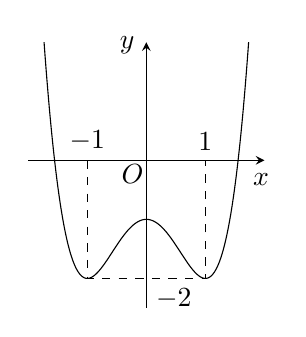
\begin{tikzpicture}[line cap=butt,line join=miter,>=stealth,scale=0.75]
		\tikzset{declare function={xmin=-2;xmax=2;ymin=-2.5;ymax=2;f(\x)=(\x)^4-2*(\x)^2-1;},smooth,samples=450}
		\draw[->] (xmin,0)--(xmax,0) node[shift={(-100:7pt)},font=\normalsize]{$ x $};
		\draw[->] (0,ymin)--(0,ymax) node[shift={(190:7pt)},font=\normalsize]{$ y $};
		\fill (0,0) node[shift={(225:7pt)},font=\normalsize]{$ O $};
		\clip (xmin,ymin) rectangle (xmax,ymax);
		\draw  plot[domain=-1.75:1.75] (\x, {f(\x)});
		\draw[dashed] (-1,0)node[above]{$-1$}--(-1,{f(-1)})--(1,{f(1)})--(1,0)node[above]{$1$};
		\node[below right] at (0,-2){$-2$};
\end{tikzpicture}}
\loigiai{
Dựa vào đồ thị, hàm số đã cho nghịch biến trên khoảng $(-1;0)$.
}
\end{ex}

%%==========Câu 25
\begin{ex}%[Dự án 12-Vted-2022, Tin Dat Tran]%[2D3B1-1]
Cho hàm số $f(x)=2 x+\sin x$. Khẳng định nào dưới đây đúng?
\choice
{$\displaystyle\int f(x) \mathrm{\,d}x=2+\cos x+C$}
{$\displaystyle\int f(x) \mathrm{\,d}x=x^2+\cos x+C$}
{\True $\displaystyle\int f(x) \mathrm{\,d}x=x^2-\cos x+C$}
{$\displaystyle\int f(x) \mathrm{\,d}x=-\cos x+C$}
\loigiai{
Ta có $\displaystyle\int f(x) \mathrm{\,d}x=\displaystyle\int \left(2x+\sin x\right) \mathrm{\,d}x =\displaystyle\int 2x \mathrm{\,d}x +\displaystyle\int \sin x \mathrm{\,d}x =x^2-\cos x +C$.
}
\end{ex}

%%==========Câu 26
\begin{ex}%[Dự án 12-Vted-2022, Tin Dat Tran]%[2H3B1-1]
Trong không gian $O x y z$, cho hai điểm $A(1 ; 0 ; 0)$ và $B(4 ; 1 ; 2)$. Toạ độ véctơ $\overrightarrow{O A}-\overrightarrow{O B}$ là
\choice
{$(5 ; 1 ; 2)$}
{\True $(-3 ;-1 ;-2)$}
{$(3 ; 1 ; 2)$}
{$(-5 ;-1 ;-2)$}
\loigiai{
Ta có 
$\heva{& \overrightarrow{OA}=(1;0;0)\\ & \overrightarrow{OB}=(4;1;2)}
\Rightarrow \overrightarrow{O A}-\overrightarrow{O B}=(-3;-1;-2)$.
}
\end{ex}

%%==========Câu 27
\begin{ex}%[Dự án 12-Vted-2022, Tin Dat Tran]%[1H3B5-3]
\immini{
Cho hình lăng trụ đứng $A B C \cdot A' B' C'$ có đáy $A B C$ là tam giác đều và $A B=4$ (tham khảo hình bên). Khoảng cách từ $C$ đến mặt phẳng $\left(A B B' A'\right)$ bằng
\choice
{$2 \sqrt{2}$}
{$2$}
{\True $2 \sqrt{3}$}
{$4$}
}{
\begin{tikzpicture}[scale=0.75]
		\def\r{3}
		\def\h{3}
		\path (0,0) coordinate (A) (\r,0) coordinate (C) (-30:0.8*\r) coordinate (B);
		\foreach \x in {A,B,C}{\path ($(\x)+(0,\h)$)coordinate (\x');\draw (\x)--(\x');}
		\draw (A)--(B)--(C) (A')--(B')--(C')--cycle;
		\draw[dashed] (A)--(C);
		\foreach \x/\y in {A/180,B/-90,C/0,A'/180,B'/90,C'/0}{\fill (\x) circle (1pt); \node at ($(\x)+(\y:.35)$){$\x$};}
\end{tikzpicture}}
\loigiai{
\immini
{Gọi $M$ là trung điểm của $A'B'$. Khi đó ta có $C'M\perp A'B'$ (do tam giác $A'B'C'$ đều).\\
Mà $AA'\perp C'M$ (Do $AA'\perp (A'B'C')$) nên $C'M\perp \left(AA'B'B\right)$.\\
$\Rightarrow\mathrm{d}\left(C',(ABB'A')\right)=C'M=4\cdot \dfrac{\sqrt{3}}{2}=2\sqrt{3}$.

}
{\begin{tikzpicture}
		\def\r{3}
		\def\h{3}
		\path (0,0) coordinate (A) (\r,0) coordinate (C) (-30:0.8*\r) coordinate (B);
		\foreach \x in {A,B,C}{\path ($(\x)+(0,\h)$)coordinate (\x');\draw (\x)--(\x');}
		\draw (A)--(B)--(C) (A')--(B')--(C')--cycle;
		\draw[dashed] (A)--(C);
		\path  ($(A')!.5!(B')$) coordinate (M);
		\draw (C')--(M); 
		\pic[draw, angle radius=8pt]{right angle=B'--M--C'};
		\foreach \x/\y in {A/180,B/-90,C/0,A'/180,B'/90,C'/0,M/-90}{\fill (\x) circle (1pt); \node at ($(\x)+(\y:.35)$){$\x$};}
\end{tikzpicture}}
}
\end{ex}

%%==========Câu 28
\begin{ex}%[Dự án 12-Vted-2022, Tin Dat Tran]%[2H2B2-4]
Một cốc nước hình trụ chứa sẵn một lượng nước có bán kính đáy $r$ và chiều cao $h=2 r$. Thả vào cốc một viên bi sắt hình cầu bán kính $r$ thì mực nước trong cốc dâng lên vừa đúng mép cốc. Thể tích nước có sẵn trong cốc là (bỏ qua độ dày của đáy và thành cốc)
\choice
{$\dfrac{1}{3} \pi r^3$}
{$\pi r^3$}
{\True $\dfrac{2}{3} \pi r^3$}
{$\dfrac{4}{3} \pi r^3$}
\loigiai{
$V_{\text{nước}}=V_\text{trụ}-V_{\text{viên bi}}=\pi\cdot  r^2\cdot 2r-\dfrac{4}{3}\pi r^3=\dfrac{2}{3}\pi r^3$.
}
\end{ex}


%%==========Câu 29
\begin{ex}%[Dự án 12-Vted-2022, Trần Thị Hồng]%[2D1B3-1]%
Trên đoạn $[0;7]$, hàm số $y=2x-3+\dfrac{8}{x+1}$ đạt giá trị lớn nhất tại điểm
\choice
{\True $x=7$}
{ $x=3$}
{$x=1$}
{$x=0$}
\loigiai{ Ta có $y'=2-\dfrac{8}{(x+1)^2}\Rightarrow y'=0\Leftrightarrow\hoac{&x=1\in[0;7]\\&x=-3\notin[0;7]}$.\\
	Lại có $y(0)=5; y(1)=3, y(7)=12$.\\
	Vậy hàm số $y=2x-3+\dfrac{8}{x+1}$ đạt giá trị lớn nhất tại điểm $x=7$.

}
\end{ex}


%%==========Câu 30
\begin{ex}%[Dự án 12-Vted-2022, Trần Thị Hồng]%[2D1K1-2]% 
	\immini{	
	Cho hàm số $y=a x^4+b x^2+c$ có đồ thị như hình vẽ bên.
	Khẳng định nào dưới đây \textbf{đúng}?
	\choice
	{$f'(1)>0$ }
	{$f'(-1)<0$}
	{$f'(1)=0$}
	{\True $f'(-1)>0$}}
{	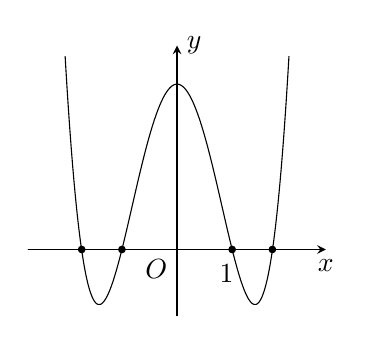
\begin{tikzpicture}[scale=0.7, line join=round, line cap=round, >=stealth]
			\tikzset{every node/.style={scale=1}}
			\def\xmin{-2.5}\def\xmax{2.5}\def\ymin{-1}\def\ymax{3.5}
			\draw[->] (\xmin-0.2,0)--(\xmax+0.2,0) node[below]{$x$};
			\draw[->] (0,\ymin-0.2)--(0,\ymax+0.2) node[right]{$y$};
			\draw (0,0) node[below left]{$O$};
			\clip (\xmin,\ymin) rectangle (\xmax,\ymax);
			\draw[smooth,samples=200,domain=\xmin:\xmax] plot (\x,{1*((\x)^4)-4*(\x)^2+3});
			\fill (-1.73,0)circle(2pt);
			\fill (1.73,0)circle(2pt);
			\fill (-1,0)circle(2pt);\fill (1,0)circle(2pt);
			\draw (1.2,-0.1) node[ below left]{$1$};
		\end{tikzpicture}
}
\loigiai{ Dựa vào đồ thị của hàm số ta thấy hàm số đồng biến trên khoảng $(x_1;0)$ với $x_1<-1$. Do đó $f'(-1)>0$.

}
\end{ex}

%%==========Câu 31
\begin{ex}%[Dự án 12-Vted-2022, Trần Thị Hồng]%[2D2K3-2]%
Với $a, b$ là các số thực dương thỏa mãn $\log _2\left(a b^3\right)=1$ và $\log _4\left(a^4 b\right)=2$, khẳng định nào dưới đây \textbf{đúng}?
\choice
{  $a^5 b^4=16$}
{  $a^3=2 b^2$}
{ $a^5 b^4=1$}
{\True $a^3=8 b^2$}
\loigiai{
Với $a, b$ là các số thực dương ta có:\\
 $\heva{&\log _2\left(a b^3\right)=1\\&\log _4\left(a^4 b\right)=2}\Leftrightarrow \heva{&a b^3=2\\&a^4 b=16}\Leftrightarrow a^3=8 b^2$.
}
\end{ex}

%%==========Câu 32
\begin{ex}%[Dự án 12-Vted-2022, Trần Thị Hồng]%[2H3B2-3]%
Trong không gian $O x y z$, mặt phẳng đi qua điểm $M(1 ; 0 ; 6)$ và song song với mặt phẳng $(\alpha)\colon x+2 y+2 z-1=0$ có phương trình là
\choice
{ $x+2 y+2 z+14=0$}
{\True $x+2 y+2 z-13=0$}
{ $x+2 y+2 z+13=0$}
{$x+2 y+2 z-14=0$}
\loigiai{
Ta có $\vv{n}_{(\alpha)}=(1;2;2)$.\\
Mặt phẳng đi qua điểm $M(1 ; 0 ; 6)$ và song song với mặt phẳng $(\alpha)$ nhận $\vv{n}_{(\alpha)}$ làm vectơ pháp tuyến có phương trình là
$$ 1\cdot (x-1)+2\cdot (y-0)+2\cdot (z-6)=0\Leftrightarrow x+2y+2z-13=0.$$

}
\end{ex}

%%==========Câu 33
\begin{ex}%[Dự án 12-Vted-2022, Trần Thị Hồng]%[2D3B2-1]%
Nếu $\displaystyle\int\limits_1^3\left[f(x)+4 x^3\right] \mathrm{d\,}x=100$ thì $\displaystyle\int\limits_1^3 f(x)\mathrm{d\,} x$ bằng
\choice
{\True $20$}
{$122$}
{$122$}
{$22$}
\loigiai{ Ta có $\displaystyle\int\limits_1^3\left[f(x)+4 x^3\right]\mathrm{d\,} x=100\Leftrightarrow \displaystyle\int\limits_1^3f(x)\mathrm{d\, } x+\displaystyle\int\limits_1^34 x^3\mathrm{d\,} x =100\Leftrightarrow \displaystyle\int\limits_1^3f(x)\mathrm{d\,} x+80=100 \Leftrightarrow \displaystyle\int\limits_1^3f(x)\mathrm{d\,} x=20$.
}
\end{ex}


%%==========Câu 34
\begin{ex}%[Dự án 12-Vted-2022, Trần Thị Hồng]%[1H3K4-3]%
\immini{
Cho hình hộp chữ nhật $ABCD.A' B' C' D'$ có đáy $ABCD$ là hình vuông cạnh bằng $2 \sqrt{2}$, $A A'=4$ (tham khảo hình bên). Góc giữa đường thẳng $A C$ và mặt phẳng $\left(A A' B' B\right)$ bằng
\choice
{ $30^{\circ}$ }
{\True $60^{\circ}$}
{ $45^{\circ}$}
{$90^{\circ}$ }
}{
	\begin{tikzpicture}[scale=.7, font=\footnotesize, line join=round, line cap=round, >=stealth]
	\def\bc{5} % cạnh BC
	\def\ba{2} % cạnh BA
	\def\bh{3} % cạnh BA
	\def\gocB{35} % góc B của đáy
	\coordinate[label=below left:$B$] (B) at (0,0);
	\coordinate[label=above left:$A$] (A) at (\gocB:\ba);
	\coordinate[label=below:$C$] (C) at (\bc,0);
	\coordinate[label=right:$D$] (D) at ($(C)-(B)+(A)$);
	\coordinate[label=above left:$A'$] (A') at ($(A)+(90:\bh)$);
	\coordinate[label=left:$B'$] (B') at ($(B)-(A)+(A')$);
	\coordinate[label=below right:$C'$] (C') at ($(C)-(A)+(A')$);
	\coordinate[label=right:$D'$] (D') at ($(D)-(A)+(A')$);
	\draw (B')--(B)--(C)--(D)--(D')--(A')--(B')--(C')--(D') (C)--(C');
	\draw[dashed] (C)--(A')--(A)--(D) (A)--(B) (A')--(B);
	\foreach \diem in {A,B,C,D,A',B',C',D'}	\fill (\diem)circle(1.5pt);
\end{tikzpicture}
}
\loigiai{
\immini{
Ta có $BC\perp (ABB'A')$ nên suy ra góc giữa đường thẳng $A' C$ và mặt phẳng $\left(A A' B' B\right)$ là $(CA, BA')=\widehat{CA'B}$.\\
Ta có $\heva{& A'B^2=AB^2+AA'^2=24\\& A'C^2=A'A^2+AC^2=16+16=32.}$\\
Suy ra 
\[\cos\widehat{CA'B}=\dfrac{A'B^2+ A'C^2-BC^2}{2A'B\cdot A'C }=\dfrac{24+32-8}{2\sqrt{24}\cdot\sqrt{32}}=\dfrac{\sqrt{3}}{2}.\]
Suy ra $\widehat{CA'B}=60^{\circ}$.\\
Vậy góc giữa đường thẳng $A' C$ và mặt phẳng $\left(A A' B' B\right)$ bằng $60^{\circ}$.

}{
	\begin{tikzpicture}[scale=.7, font=\footnotesize, line join=round, line cap=round, >=stealth]
	\def\bc{5} % cạnh BC
	\def\ba{2} % cạnh BA
	\def\bh{3} % cạnh BA
	\def\gocB{35} % góc B của đáy
	\coordinate[label=below left:$B$] (B) at (0,0);
	\coordinate[label=above left:$A$] (A) at (\gocB:\ba);
	\coordinate[label=below:$C$] (C) at (\bc,0);
	\coordinate[label=right:$D$] (D) at ($(C)-(B)+(A)$);
	\coordinate[label=above left:$A'$] (A') at ($(A)+(90:\bh)$);
	\coordinate[label=left:$B'$] (B') at ($(B)-(A)+(A')$);
	\coordinate[label=below right:$C'$] (C') at ($(C)-(A)+(A')$);
	\coordinate[label=right:$D'$] (D') at ($(D)-(A)+(A')$);
	\draw (B')--(B)--(C)--(D)--(D')--(A')--(B')--(C')--(D') (C)--(C');
	\draw[dashed] (C)--(A')--(A)--(D) (A)--(B) (A')--(B);
	\foreach \diem in {A,B,C,D,A',B',C',D'}	\fill (\diem)circle(1.5pt);
\end{tikzpicture}
}
}
\end{ex}

%%==========Câu 35
\begin{ex}%[Dự án 12-Vted-2022, Trần Thị Hồng]%[2D4B2-1]%
Cho hai số thực $a, b$ thỏa mãn $a+b i=(1+i) \cdot i$, (trong đó $i$ là đơn vị ảo). Giá trị của $a+b$ bằng
\choice
{\True $0$}
{ $ 2$}
{ $-1+i$ }
{ $1+i$}
\loigiai{
Ta có $(1+i) \cdot i=-1+i$.\\ 
Do đó $a=-1, b=1 \Rightarrow a+b=0$.
}
\end{ex}

%%==========Câu 36
\begin{ex}%[Trương Đăng Khoa]%[Đề Vted 14]%[2D1B5-4]
	Cho hàm số $y=f(x)$ có bảng biến thiên như hình vẽ
	\begin{center}
		
\begin{tikzpicture}[scale=1, font=\footnotesize]
			\tkzTabInit[nocadre=false, lgt=1.2, espcl=2, deltacl=0.6]
			{$x$/0.8,$f'(x)$/0.6,$f(x)$/2}
			{$-\infty$,$-2$,$0$,$1$,$+\infty$};
			\tkzTabLine{,+,$0$,-,d,-,$0$,+,};
			\tkzTabVar{-/$-5$,+/$1$,-D+/$-2$/$+\infty$,-/$3$,+/$5$};
		\end{tikzpicture}
	\end{center}
	Số giá trị nguyên của tham số $m$ để phương trình $f(x)=m$ có đúng hai nghiệm phân biệt là
	\choice
	{$2$}
	{$3$}
	{$5$\True}
	{$4$}
	\loigiai
	{
Phương trình $f(x)=m$ có hai nghiệm phân biệt khi 	$\hoac{&-2\leq m<1\\ &3<m\leq 5}$.\\
Mà $m\in\mathbb{Z}\Rightarrow m\in\{-2;-1;0;4;5\}$.
}
\end{ex}

%%==========Câu 37
\begin{ex}%[Trương Đăng Khoa]%[Đề Vted 14]%[1D2B5-5]
	Từ một hộp chứa $16$ quả cầu gồm $7$ quả màu đỏ và $9$ quả màu xanh, lấy ngẫu nhiên đồng thời hai quả. Xác suất để lấy được hai quả cùng màu bằng 
	\choice 
	{$\dfrac{7}{40}$}
	{$\dfrac{21}{40}$}
	{$\dfrac{33}{40}$}
	{$\dfrac{19}{40}$\True}
	\loigiai
	{
	Số phần tử không gian mẫu là $n(\Omega)=\mathrm{C}_{16}^2$.\\
	Gọi biến cố A là \lq\lq lấy được hai quả cùng màu\rq\rq.\\
	 Trường hợp $1$. Lấy được hai quả cầu cùng màu đỏ.\\
	 Số cách chọn $2$ quả cầu đỏ là $\mathrm{C}_7^2$.\\
	 Trường hợp $2$. Lấy được hai quả cầu cùng màu xanh.\\
	 Số cách chọn $2$ quả cầu đỏ là $\mathrm{C}_9^2$.\\
	 Vậy $\mathrm{P}(A)=\dfrac{\mathrm{C}_7^2+\mathrm{C}_9^2}{\mathrm{C}_{16}^2}=\dfrac{19}{40}$.
}
\end{ex}

%%==========Câu 38
\begin{ex}%[Trương Đăng Khoa]%[Đề Vted 14]%[2D3K1-1]
	Biết $F(x)=x^{\tfrac{3}{2}}$ là một nguyên hàm của $\dfrac{f(x)}{x^2}$ trên $(0;+\infty)$. Hàm số nào dưới đây là nguyên hàm của $f(x)$ trên $(0;+\infty)$?
	\choice 
	{$\dfrac{3}{7} x^{\tfrac{7}{2}}+C$\True}
	{$\dfrac{2}{9} x^{\tfrac{9}{2}}+C$}
	{$\dfrac{3}{2} x^{\tfrac{5}{2}}+C$}
	{$\dfrac{3}{5} x^{\tfrac{7}{2}}+C$}
	\loigiai{
Ta có $\displaystyle\int \dfrac{f(x)}{x^2}\mathrm{d\,}x=F(x)\Rightarrow \dfrac{f(x)}{x^2}=F'(x)=\left(x^{\tfrac{3}{2}} \right)'=\dfrac{3}{2}\cdot \dfrac{x^{\tfrac{5}{2}}}{x^2}\Rightarrow f(x)=\dfrac{3}{2}\cdot x^{\tfrac{5}{2}}$.\\
Vậy $ \displaystyle\int f(x)\mathrm{d\,}x= \displaystyle\int \dfrac{3}{2}\cdot x^{\tfrac{5}{2}}\mathrm{d\,}x=\dfrac{3}{7}\cdot x^{\tfrac{7}{2}}+C$.
}
\end{ex}

%%==========Câu 39
\begin{ex}%[Trương Đăng Khoa]%[Đề Vted 14]%[2D2K6-3]
	Có bao nhiêu số nguyên $x$ thỏa mãn $\log_3^2\left(3x^2\right)-8\log_3|x|\le 9$?
	\choice 
	{$18$\True}
	{$7$}
	{$19$}
	{$9$}
	\loigiai{
Ta xét $\begin{aligned}[t]
	&\log_3^2\left(3x^2\right)-8\log_3|x|\le 9\\
	\Leftrightarrow& \left(1+2\log_3 |x|\right)^2-8\log_3|x|\le 9.\\
\end{aligned}	$\\
Đặt $\log_3|x|=a$ khi đó 
\allowdisplaybreaks
$\begin{aligned}[t]
	&\left(1+2\log_3 |x|\right)^2-8\log_3|x|\le 9\\
	\Leftrightarrow& (1+2a)^2-8a\le 9
	\Leftrightarrow  4a^2-4a-8\leq 0
	\Leftrightarrow -1\leq a\leq 2
	\Leftrightarrow -1 \leq \log_3|x|\leq 2
	\Leftrightarrow& \dfrac{1}{3}\leq |x| \leq 9\\
	\Leftrightarrow& \heva{&|x|\leq 9\\
	 &|x|\geq \dfrac{1}{3}}
 \Leftrightarrow  \heva{&-9\leq x \leq 9\\ &\hoac{&x\geq \dfrac{1}{3}\\ & x\leq -\dfrac{1}{3}}}
 \Leftrightarrow  \hoac{ & \dfrac{1}{3}\leq x\leq 9\\ &-9\leq x\leq -\dfrac{1}{3}}.
\end{aligned}$\\
Mà $x\in\mathbb{Z}$.
Vậy phương trình có $18$ nghiệm nguyên.
}
\end{ex}

%%==========Câu 40
\begin{ex}%[Trương Đăng Khoa]%[Đề Vted 14]%[2H3K2-3]
	Trong không gian $O x y z$, cho ba điểm $A(2;3;-1)$, $B(1;1;0)$, $C(4;7;3)$. Gọi $(P)$ là mặt phẳng qua $A$, trực tâm của tam giác $ABC$ và vuông góc với mặt phẳng $(ABC)$. Điểm nào dưới đây thuộc $(P)$?
	\choice 
	{$Q(-2;-2;-1)$}
	{$M(1;-3;-2)$}
	{$N(1;2;2)$\True}
	{$P(-8;0;3)$}
	\loigiai
	{
Ta không cần tìm trực tâm $H$ của tam giác $ABC$.\\
Mặt phẳng cần tìm là mặt phẳng chứa $AH$ và vuông góc với mặt phẳng $(ABC)$.\\ 
Vì $BC\perp AH=(P)\cap (ABC)$; $(P)\perp(ABC)\Rightarrow BC\perp (P)$.\\
Do đó véc-tơ pháp tuyến $\vec{n}_P=\vv{BC}=(3;6;3)=3 (1;2;1)\Rightarrow (P)\colon x+2y+z-7=0$ qua điểm $N(1;2;2)$.
}
\end{ex}


%----Câu 41
\begin{ex}%[Phan Quốc Trí, Đề-Vted-đợt-2]%[2D3K2-4]
Cho hàm số $f(x)$ có đạo hàm $f'(x)=\mathrm{e}^x \sin x+2 x-1,~ \forall x \in \mathbb{R}$ và $f(0)=1$. Gọi $F$ là một nguyên hàm của $f$ trên $\mathbb{R}$ sao cho $F(0)=-1$, khi đó $F(1)$ bằng
\choice
{\True $\dfrac{1}{6}(5-3\mathrm{e} \cos 1)$}
{$\dfrac{1}{6}(7-3\mathrm{e} \cos 1)$}
{$\dfrac{1}{6}(5+3\mathrm{e}\cos 1)$}
{$-\dfrac{1}{6}(7+3\mathrm{e} \cos 1)$}
\loigiai{
	\begin{eqnarray*}
		F(1)&= &F(0)+\int_0^1 f(x) \mathrm{\,d}x=-1+\int_0^1 f(x) \mathrm{\,d}x=-1+\int_0^1 f(x) \mathrm{\,d}(x-1) \\
		&=&-1+(x-1) f(x)\Bigg|_0 ^1-\int_0^1(x-1) f'(x) \mathrm{\,d}x  \\
		&=& -1+1-\int_0^1(x-1)\left(\mathrm{e}^x \sin x+2 x-1\right) \mathrm{\,d}x=\dfrac{1}{6}\left(5-3\mathrm{e} \cos 1\right).
	\end{eqnarray*}
}
\end{ex}
%----Câu 42
\begin{ex}%[Phan Quốc Trí, Đề-Vted-đợt-2]%[2H2K1-1]
Cho hình trụ $(T)$ có $O$, $O'$ lần lượt là tâm hai đường tròn đáy. Tam giác $ABC$ nội tiếp trong đường tròn tâm $O$, $AB=2a$, $\sin \widehat{ACB}=\dfrac{1}{\sqrt{3}}$ và $OO'$ tạo với mặt phẳng $\left(O'AB\right)$ một góc $30^{\circ}$. Thể tích khối trụ $(T)$ bằng
\choice
{\True $3 \pi a^3 \sqrt{6}$}
{$\pi a^3 \sqrt{3}$}
{$\pi a^3 \sqrt{6}$}
{$2 \pi a^3 \sqrt{6}$}
\loigiai{
\immini{
Bán kính đường tròn đáy $r$ của $(T)$ chính là bán kính đường tròn ngoại tiếp tam giác $ABC$ và $$r=\dfrac{AB}{2\sin\widehat{ACB}}=\dfrac{2a}{2\cdot\dfrac{1}{\sqrt{3}}}=\sqrt{3}a.$$
Gọi $M$ là trung điểm $AB$
$$\Rightarrow OM=\sqrt{OA^2- AM^2}=\sqrt{(\sqrt{3} a)^2-a^2}=\sqrt{2} a.$$
Và $\left(OO',\left(O'AB\right)\right)=\widehat{OO'M}=30^{\circ} \Rightarrow h=OO'=OM\cdot \cot 30^\circ=\sqrt{6}a$.\\
Vậy $V_{(T)}=\pi r^2 h=\pi\cdot \left(\sqrt{3} a\right)^2 \cdot \sqrt{6} a=3 \sqrt{6} \pi a^3$.
}{
\begin{tikzpicture}[scale=1,>=stealth, font=\footnotesize, line join=round, line cap=round]
	\def \x{2.4} %bán kính trục lớn elip
	\def \y{1} %bán kính trục bé elip
	\def \h{3} %chiều cao hình trụ
	\coordinate (P) at (0,0);
	\coordinate (N) at (2*\x,0);
	\coordinate (O) at ($(P)!0.5!(N)$);
	\coordinate (O') at ($(O)+(0,\h)$);
	\coordinate (P') at ($(P)+(0,\h)$);
	\coordinate (N') at ($(N)+(0,\h)$);
	%Lấy các điểm A,B trên elip
	\coordinate (A) at ($(O)+({\x*cos(80)},{\y*sin(80)})$);
	\coordinate (B) at ($(O)+({\x*cos(-30)},{\y*sin(-30)})$);
	\coordinate (C) at ($(O)+({\x*cos(-150)},{\y*sin(-150)})$);
	\coordinate (M) at ($(A)!0.5!(B)$);
	\draw[dashed] (N) arc(0:180:\x cm and \y cm);
	\draw (N) arc(0:-180:\x cm and \y cm);
	\draw (O') ellipse (\x cm and \y cm);
	\draw (P)--(P') (N)--(N');
	\draw[dashed]
	(O)--(O')--(M)--(O)
	(B)--(O')--(A)--(O)
	(A)--(B)--(C)--cycle
	;
	\foreach \p/\r in {O/-90,O'/90,A/135,B/-90,C/-135,M/-90}
	\fill (\p) circle (1pt) node[shift={(\r:3mm)}]{$\p$};
	\draw (O')pic[fill=yellow,draw=black, angle eccentricity=1.35, angle radius=0.6cm]{angle=O--O'--M}
	;
	\foreach \p/\r/\t in{O/M/A}
	\draw pic[fill=blue!30,draw=black, angle eccentricity=0.75, angle radius=0.2cm]{right angle=\p--\r--\t};
\end{tikzpicture}
}
}
\end{ex}
%----Câu 43
\begin{ex}%[Phan Quốc Trí, Đề-Vted-đợt-2]%[2D4G5-1]
Xét hai số phức $z_1$, $z_2$ thoả mãn $\left|z_1-z_2\right|=\left|z_1-3 i\right|$; $\left|z_2+2-i\right|=4$ và $\left(z_1+2-i\right) \overline{\left(z_1-z_2\right)}$ là một số thực. Gọi $M$, $m$ lần lượt là giá trị lớn nhất, giá trị nhỏ nhất của biểu thức $P=\left|z_2-z_1\right|$, giá trị của $M^2+m^2$ bằng
\choice
{$8\sqrt{2}$}
{\True $12$}
{$16$}
{$4\sqrt{2}$}
\loigiai{
\immini{ Gọi $M$, $N$, $A$ lần lượt là điểm biểu diễn của các số phức $z_1$, $z_2$, $3 i$.\\
$\Rightarrow\left|z_1-z_2\right|=\left|z_1-3 i\right| \Leftrightarrow MN=MA$ và $\left|z_2+2-i\right|=4$ $\Rightarrow N \in (C)$ có tâm $I(-2;1)$, $R=4$.\\
Đặt $z_1=x+yi$, $z_2=x'+y'i$. Ta có $\overrightarrow{IM}=(x+2;y-1)$ , $\overrightarrow{MN}=(x'-x;y'-y)$ và 
$	\left(z_1+2-i\right) \overline{\left(z_1-z_2\right)} = \left[x+2 +(y-1)i\right]\cdot \left[x-x'-(y-y')i\right] $ là số thực nên 
\begin{eqnarray*}
(x-x')(y-1)-(x+2)(y-y')=0
\end{eqnarray*}
do đó $I$, $M$, $N$ thẳng hàng do đó $M$ là giao của $IN$ với trung trực đoạn $AN$.
}{
\begin{tikzpicture}[scale=0.8,>=stealth, font=\footnotesize, line join=round, line cap=round]
	\foreach \i/\j/\k in{0/0/I,3/0/N,1/1.7/A}
	\coordinate (\k) at(\i,\j);
	\coordinate (H) at($(A)!0.5!(N)$);
	\path
	($(H)!1!90:(N)$) coordinate (h1)
	(intersection of H--h1 and I--N) coordinate (M);
	\draw(A)--(I)--(N)--cycle
	;
	\draw (I) circle (3 cm);
	\coordinate (A1) at($(A)!0.5!(I)$);
	\draw[rotate=59.5] (A1) ellipse (1.7 cm and 1.12 cm);
	\draw (A)--(M)--(H);
	\foreach \p/\r in {A/90,I/-135,N/0,H/45,M/-90}
	\fill (\p) circle (1pt) node[shift={(\r:3mm)}]{$\p$};
	\foreach \p/\r/\t in{A/H/M}
	\draw pic[draw=black, angle eccentricity=0.75, angle radius=0.1cm]{right angle=\p--\r--\t};
\end{tikzpicture}
}
\noindent Do đó $MI+MA=MI+MN=IN=4$.
$\Rightarrow M \in(E)$ có hai tiêu điểm $I$, $A$; độ dài trục lớn $2a=4$; tiêu cự $2c=IA=2 \sqrt{2}$; độ dài trục nhỏ $2b=2 \sqrt{a^2-c^2}=2\sqrt{2}$.
\immini{
	Ta có $P=\left|z_2-z_1\right|=MN=IN-IM=4-IM$.\\
	Và $IM \geq I A_2=E A_2-E I=a-c=2-\sqrt{2}$;\\ $IM \leq IA_1=EI+EA_1=a+c=2+\sqrt{2}$.\\
	$\Rightarrow$ $M=2+\sqrt{2}$; $m=2-\sqrt{2}$ $\Rightarrow M^2+m^2=12$.
}{
	\begin{tikzpicture}[scale=1,>=stealth, font=\footnotesize, line join=round, line cap=round]
	\foreach \i/\j/\k in{0/0/E,2/0/A_1,-2/0/A_2}
	\coordinate (\k) at(\i,\j);
	\coordinate (I) at ($(A_2)!0.2!(A_1)$);
	\coordinate (A) at ($(A_2)!0.8!(A_1)$);
	\draw (E) ellipse (2 cm and 1 cm);
	\coordinate (M) at ($(E)+({2*cos(100)},{1*sin(100)})$);
	\draw (A_2)--(A_1)(I)--(M);
	\foreach \p/\r in {A_2/-150,A_1/-30,E/-90,M/90,A/-90,I/-90}
	\fill (\p) circle (1pt) node[shift={(\r:3mm)}]{$\p$};
\end{tikzpicture}
}
}
\end{ex}
%----Câu 44
\begin{ex}%[Phan Quốc Trí, Đề-Vted-đợt-2]%[2H1K3-4]
Cho khối chóp $S.ABCD$ có đáy là hình vuông cạnh $a$. Cạnh bên $SA$ vuông góc với mặt đáy. Gọi $H$, $K$ lần lượt là hình chiếu vuông góc của $A$ lên $SB$ và $SD$; góc giữa hai mặt phẳng $(ABCD)$ và $(AHK)$ bằng $30^{\circ}$. Thể tích khối chóp đã cho bằng
\choice
{$\dfrac{a^3 \sqrt{2}}{3}$}
{$\dfrac{a^3 \sqrt{6}}{2}$}
{\True $\dfrac{a^3 \sqrt{6}}{3}$}
{$\dfrac{a^3 \sqrt{6}}{9}$}
\loigiai{
\immini{
Ta có $BC \perp(SAB) \Rightarrow BC \perp AH \Rightarrow AH \perp(SBC) \Rightarrow AH \perp SC$.\\
Tương tự $CD \perp(SAD) \Rightarrow CD \perp AK \Rightarrow A K \perp(S C D) \Rightarrow AK \perp SC$.\\
Do đó $SC \perp(AHK) \Rightarrow \left((ABCD),(AHK)\right)=(SA,SC)=\widehat{A SC}=30^\circ$.\\
$\Rightarrow SA=AC\cdot \cot 30^\circ=\sqrt{6}a$.\\
Vậy $V_{S.ABCD}=\dfrac{1}{3} \cdot a^2 \cdot \sqrt{6} a=\dfrac{\sqrt{6} a^3}{3}$.
}{
\begin{tikzpicture}[scale=0.8,>=stealth, font=\footnotesize, line join=round, line cap=round]
	\coordinate (A) at (0,0);
	\coordinate (B) at (-1.3,-1.6);
	\coordinate (D) at (3.5,0);
	\coordinate (C) at ($(B)+(D)-(A)$);
	\coordinate (S) at ($(A)+(0,2.6)$);
	\coordinate (H) at ($(S)!0.4!(B)$);
	\coordinate (K) at ($(S)!0.4!(D)$);
	\draw (S)--(B)--(C)--(D)--cycle;
	\draw (S)--(B) (S)--(C);
	\draw[dashed] (A)--(B) (A)--(D) (S)--(A)
	(A)--(H)--(K)--cycle
	;
	\foreach \p/\r in {S/90,A/-45,B/-90,C/-45,D/0,H/180,K/45}
	\fill (\p) circle (1pt) node[shift={(\r:3mm)}]{$\p$};
\end{tikzpicture}
}
}
\end{ex}
%----Câu 45
\begin{ex}%[Phan Quốc Trí, Đề-Vted-đợt-2]%[2D1G5-3]
	\immini{
	Cho hàm số $f(x)$ liên tục trên $\mathbb{R}$ và có đồ thị như hình bên. Xét \break $T=2f\left(a^2+a+1\right)+3f\left(a^2f(a)+b^2f(b)\right)$, $a,b \in \mathbb{R}$. Có bao nhiêu cặp số thực $\left(a;b\right)$ để $T=30$?
	\choice
	{$10$}
	{$4$}
	{$6$}
	{\True $8$}
}{
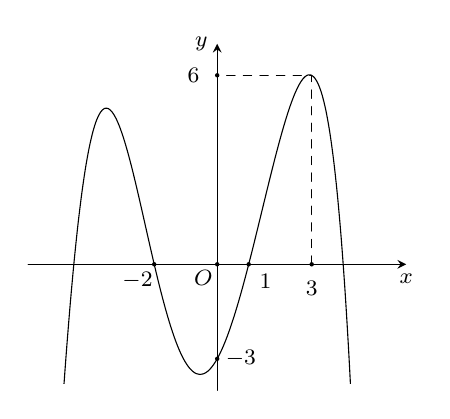
\begin{tikzpicture}[scale=0.8,>=stealth, font=\footnotesize, line join=round, line cap=round]
	\def\xmin{-3} \def\xmax{3}
	\def\ymin{-2} \def\ymax{3.5}
	%\draw[color=gray!50,dashed] (\xmin,\ymin) grid (\xmax,\ymax);
	\draw[->] (\xmin,0)--(\xmax,0) node [below]{$x$};
	\draw[->] (0,\ymin)--(0,\ymax) node [left]{$y$};
	\fill (0,0) circle (1pt) node[shift={(-135:2.5mm)}]{$O$};
	\clip (\xmin+0.1,\ymin+0.1) rectangle (\xmax-0.5,\ymax-0.1);
	\draw[smooth,samples=100,domain=-3:3] plot(\x,{0-0.021531945652311417*(\x)^(7.0)-0.03230227018569434*(\x)^(6.0)+0.18116264479835498*(\x)^(5.0)-0.4625042515560918*(\x)^(4.0)-0.9526579677777988*(\x)^(3.0)+2.991853329195477*(\x)^(2.0)+1.7900740760854459*(\x)-1.5});
	\fill (-1,0) circle (1pt) node[shift={(-135:3mm)}]{$-2$};
	\fill (0.5,0) circle (1pt) node[shift={(-45:3mm)}]{$1$};
	\fill (1.5,0) circle (1pt) node[shift={(-90:3mm)}]{$3$};
	\fill (0,3) circle (1pt) node[shift={(180:3mm)}]{$6$};
	\fill (0,-1.5) circle (1pt) node[shift={(0:3mm)}]{$-3$};
	\draw[dashed] (1.5,0)|-(0,3);
\end{tikzpicture}
}
	\loigiai{
\immini{
Quan sát đồ thị đã cho ta có $\max\limits_{\mathbb{R}} f(x)=f(3)=6$.\\
Do đó $T \leq 2\cdot 6+3\cdot 6=30$.\\
Dấu bằng xảy ra khi và chỉ khi
$$
\heva{&a^2+a+1=3\\&a^2f(a)+b^2f (b)=3}
\Leftrightarrow 
\hoac{&
	\heva{&a=1\\&b^2f(b)=3-a^2 f(a)} \\
	&\heva{&a=-2\\&
	b^2f(b)=3-a^2f(a) }}
\Leftrightarrow \heva{&
	a \in\{-2,1\} \\
	&b^2f(b)=3.}$$
Vì $f(-2)=f(1)=0$.
}{
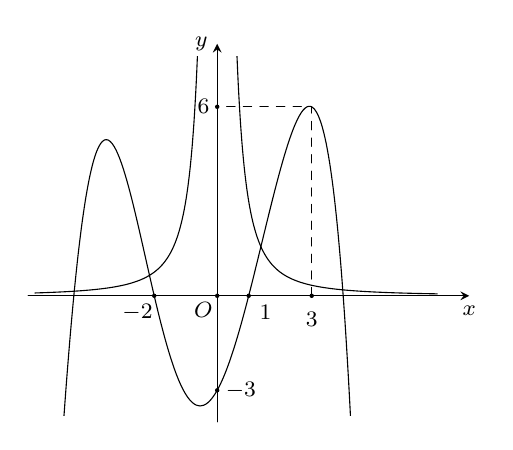
\begin{tikzpicture}[scale=0.8,>=stealth, font=\footnotesize, line join=round, line cap=round]
	\def\xmin{-3} \def\xmax{4}
	\def\ymin{-2} \def\ymax{4}
	%\draw[color=gray!50,dashed] (\xmin,\ymin) grid (\xmax,\ymax);
	\draw[->] (\xmin,0)--(\xmax,0) node [below]{$x$};
	\draw[->] (0,\ymin)--(0,\ymax) node [left]{$y$};
	\fill (0,0) circle (1pt) node[shift={(-135:2.5mm)}]{$O$};
	\clip (\xmin+0.1,\ymin+0.1) rectangle (\xmax-0.5,\ymax-0.2);
	\draw[smooth,samples=100,domain=-3:3] plot(\x,{0-0.021531945652311417*(\x)^(7.0)-0.03230227018569434*(\x)^(6.0)+0.18116264479835498*(\x)^(5.0)-0.4625042515560918*(\x)^(4.0)-0.9526579677777988*(\x)^(3.0)+2.991853329195477*(\x)^(2.0)+1.7900740760854459*(\x)-1.5});
	\draw[smooth,samples=100,domain=0.2:3.5] plot(\x,{0.375/(\x)^2});
	\draw[smooth,samples=100,domain=-3.5:-0.2] plot(\x,{0.375/(\x)^2});
	\fill (-1,0) circle (1pt) node[shift={(-135:3mm)}]{$-2$};
	\fill (0.5,0) circle (1pt) node[shift={(-45:3mm)}]{$1$};
	\fill (1.5,0) circle (1pt) node[shift={(-90:3mm)}]{$3$};
	\fill (0,3) circle (1pt) node[shift={(180:1.75mm)}]{$6$};
	\fill (0,-1.5) circle (1pt) node[shift={(0:3mm)}]{$-3$};
	\draw[dashed] (1.5,0)|-(0,3);
\end{tikzpicture}
}
\noindent Phương trình $b^2 f(b)=3 \Leftrightarrow f(b)=\dfrac{3}{b^2}\quad (\ast)$
(do $b=0$ không là nghiệm).\\
Vẽ thêm đồ thị của hàm số $y=\dfrac{3}{x^2}$ suy ra $(\ast)$ có $4$ nghiệm.\\ Vậy có tất cả $2\cdot 4=8$ cặp số $(a;b)$.
}
\end{ex}

%----Câu 46
\begin{ex}%[Đề Vted-14]%[Bùi Mạnh Tiến]%[2H3G3-8]
Trong KG $Oxyz$ cho mặt cầu $(S)\colon (x+1)^2+(y+1)^2+(z-2)^2=9$ và đường
thẳng $d\colon \dfrac{x+1}{1}=\dfrac{y-2}{-2}=\dfrac{z+1}{-2}$. Xét điểm $M$ di động trên mặt phẳng $(P)\colon 2x+2y-z-3=0$ sao cho các tiếp điểm của tiếp tuyến kẻ từ $M$ đến $(S)$ nằm trên một đường tròn có bán kính bằng $1$. Khoảng cách từ $M$ đến đường thẳng $d$ có giá trị lớn nhất bằng
\choice
{$\dfrac{3\sqrt{5}+6}{3}$}
{\True $\dfrac{12+3\sqrt{2}}{4}$}
{$\dfrac{6\sqrt{5}+15}{5}$}
{$\dfrac{3\sqrt{14}+6}{2}$}
\loigiai{
\immini{
Mặt cầu $(S)$ có tâm $I(-1;-1;2)$, bán kính $R=3$.\\
Gọi $J$ là hình chiếu vuông góc của $A$ lên $IM$.\\
Tập hợp các tiếp điểm $A$ của tiếp tuyến kẻ từ $M$ đến $(S)$ nằm trên một đường tròn tâm $J$ có bán kính bằng
\begin{align*}
JA=\dfrac{AI\cdot AM}{IM}=\dfrac{3\sqrt{x^2-9}}{x}=1\Leftrightarrow x=\dfrac{9\sqrt{2}}{4}\,\left(x=IM>3\right).
\end{align*}
Do đó $M$ thuộc mặt cầu $(T)$ có tâm $I(-1;-1;2)$, bán kính $R=\sqrt{\dfrac{81}{8}}=\dfrac{9\sqrt{2}}{4}$.
}
{
\begin{tikzpicture}[line join = round, line cap = round,>=stealth,font=\footnotesize,scale=0.65]
\def \bk{2};
\path
(0,0) coordinate (I)
(5,0) coordinate (M)
($(I)!0.5!(M)$) coordinate (N)
;
\draw [name path=c1] (I) circle (\bk);
\draw [name path=c2,color=white] (N) circle (2.5);
\path[name intersections={of=c1 and c2,by={A,B}}]; 
\path
($(I)!(A)!(M)$) coordinate (J)
;
\draw (I) -- (A) -- (M) -- (I) (A) -- (J);
\foreach \x/\g in {A/90,I/180,M/0,J/-90} \fill[black](\x) circle (1pt)+(\g:3mm) node{$\x$};
\draw pic [draw, angle radius = 2.5mm]{right angle = A--J--M};
\end{tikzpicture}
}
\noindent
Mặt khác $M\in (P)$ do đó $M\in (C)$ là đường tròn giao tuyến của $(T)$ và $(P)$ có tâm $H$ là hình chiếu vuông góc của $I$ lên $(P)$.\\
\immini{
Đường thẳng $IH$ đi qua điểm $I(-1;-1;2)$ và nhận $\overrightarrow{n}_{(P)}=(2;2;-1)$ làm véc-tơ chỉ phương có phương trình $IH\colon \heva{& x=-1+2t \\ & y=-1+2t\\&z=2-t.}$\\
Vì $H\in IH\Rightarrow H(-1+2t;-1+2t;2-t)$.\\ 
Vì $H\in (P)$ nên ta có phương trình
\begin{align*}
2(-1+2t)+2(-1+2t)-(2-t)-3=0\Leftrightarrow t=1\Rightarrow H(1;1;1).
\end{align*} 
Bán kính đường tròn $(C)$ là $R_{(C)}=\sqrt{R_{T}^2-IH^2}=\sqrt{\dfrac{81}{8}-9}=\dfrac{3\sqrt{2}}{4}$.\\
Để ý rằng $d\subset (P)$. Do đó
\begin{align*}
\mathrm{d}(M,d)=ME\leq MK\leq HK+HM=\mathrm{d}(H,d)+R_{(C)}=3+\dfrac{3\sqrt{2}}{4}=\dfrac{12+3\sqrt{2}}{4}.
\end{align*}
}{
\begin{tikzpicture}[line join = round, line cap = round,>=stealth,font=\footnotesize,scale=0.7]
\def \bk{2}
\path
(0,0) coordinate (H)
($(H)+(90:\bk)$) coordinate (M_0)
($(H)+(65:\bk)$) coordinate (M)
(-3,-3) coordinate (d')
(3,-3) coordinate (d)
($(d)!(H)!(d')$) coordinate (K)
($(d)!(M)!(d')$) coordinate (E) 
;
\draw (H) circle (\bk);
\draw (M_0) -- (K) -- (M) (H) -- (M) -- (E) (d') -- (d) node[above] {$d$};
\foreach \x/\g in {M_0/90,M/70,H/180,E/-90,K/-90} \fill[black](\x) circle (1pt)+(\g:3mm) node{$\x$};
\draw pic [draw, angle radius = 2.5mm]{right angle = H--K--E};
\draw pic [draw, angle radius = 2.5mm]{right angle = M--E--d};
\end{tikzpicture}
}
}
\end{ex}

%----Câu 47
\begin{ex}%[Đề Vted-14]%[Bùi Mạnh Tiến]%[2D2G6-5]
Có bao nhiêu số nguyên $x$ sao cho ứng với mỗi $x$, tồn tại đúng $12$ số nguyên $y$ thoả mãn 
$$6\ln \left(1+x+y\right)\geq 2xy+y^2-9y+2x^2.$$
\choice
{$7$}
{$6$}
{$9$}
{\True $8$}
\loigiai
{
Điều kiện: $1+x+y>0\Leftrightarrow y>-x-1$.\\
Xét $g(y)=2xy+y^2-9y+2x^2-6\ln (1+x+y)$ trên $(-x-1;+\infty)$ ta có
\begin{align*}
g'(y)=2x+2y-9-\dfrac{6}{1+x+y}\Rightarrow g'(y)=0\Leftrightarrow \hoac{& y=5-x \\ & y=-\dfrac{3}{2}-x<-1-x\text{ (loại)}}\Leftrightarrow y=5-x.
\end{align*}
Bảng biến thiên của hàm số $g(y)$
\begin{center}
\begin{tikzpicture}[line join = round, line cap = round,>=stealth,font=\footnotesize,scale=1]
\tkzTabInit[nocadre=false,lgt=1.2,espcl=3.5,deltacl=0.6]
{$y$ /0.6, $g’(y)$ /0.6, $g(y)$ /2}
{$-x-1$,$5-x$,$+\infty$}
\path
($(N12)!0.5!(N13)$) coordinate (d')
($(N32)!0.5!(N33)$) coordinate (d) 
;
\draw [name path=d] (d') -- (d) node[above] {$y=0$};
\draw (N12) node[below] (A) {$+\infty$} (N23) node[above] (B) {$g(5-x)$} (N32)[below] node(C)  {$+\infty$};
\draw[->,name path=d1] (A) -- (B);
\draw[->,name path=d2] (B) -- (C);
\path[name intersections={of=d and d1,by=A}]; 
\path[name intersections={of=d and d2,by=B}];
\tkzTabLine{ ,-,z,+, }
\draw[dashed] (A) -- ($(A)+(0,1.9)$) node {$a$};
\draw[dashed] (B) -- ($(B)+(0,1.9)$) node {$b$};
\end{tikzpicture}

\end{center}
Trước tiên bất phương trình phải có nghiệm tức là
\begin{align*}
g(5-x)\leq 0\Leftrightarrow 2x(5-x)+(5-x)^2-9(5-x)+2x^2-6\ln 6\leq 0\Leftrightarrow x^2+9x-20-6\ln 6\leq 0.
\end{align*}
Vì $x\in \mathbb{Z}$ nên $x\in \{-11;\ldots;2\}$. Thử với từng trường hợp ta có
\begin{multicols}{2}
\begin{itemize}
\item $x=-11\Rightarrow y\in \{14;\ldots;18\}$.
\item $x=-10\Rightarrow y\in \{11;\ldots;19\}$.
\item $x=-9\Rightarrow y\in \{9;\ldots;19\}$.
\item $x=-8\Rightarrow y\in \{8;\ldots;19\}$.
\item $x=-7\Rightarrow y\in \{7;\ldots;18\}$.
\item $x=-6\Rightarrow y\in \{6;\ldots;17\}$.
\item $x=-5\Rightarrow y\in \{5;\ldots;16\}$.
\item $x=-4\Rightarrow y\in \{4;\ldots;15\}$.
\item $x=-3\Rightarrow y\in \{3;\ldots;14\}$.
\item $x=-2\Rightarrow y\in \{2;\ldots;13\}$.
\item $x=-1\Rightarrow y\in \{1;\ldots;12\}$.
\item $x=0\Rightarrow y\in \{0;\ldots;10\}$.
\item $x=1\Rightarrow y\in \{0;\ldots;8\}$.
\item $x=2\Rightarrow y\in \{1;\ldots;5\}$.
\end{itemize}
\end{multicols}
Suy ra $x\in \{-8;\ldots;-1\}$.\\ 
Vậy có tất cả $8$ giá trị nguyên của $x$ thoả mãn yêu cầu bài toán.
}
\end{ex}


%----Câu 48
\begin{ex}%[Đề Vted-14]%[Bùi Mạnh Tiến]%[2D4G4-2]
Trên tập hợp số phức, gọi $z_1$, $z_2$ là hai nghiệm phức của phương trình $z^2+az+b=0$ và $z_3$, $z_4$ là hai nghiệm phức của phương trình $z^2+cz+d=0$ với $a$, $b$, $c$, $d\in \mathbb{Z}$. Biết rằng $z_1+z_3=3+4i$ và $z_2\cdot z_4=-8-6i$. Khi đó $ac+b+d$ bằng
\choice
{\True $9$}
{$84$}
{$41$}
{$34$}
\loigiai
{
\begin{itemize}
\item \textbf{Trường hợp 1}: Nếu cả hai phương trình đều có nghiệm thực, khi đó $z_1+z_3$ là số thực (loại).
\item \textbf{Trường hợp 2}: Nếu một phương trình có nghiệm thực và một phương trình có nghiệm không là số thực.\\
Giả sử phương trình $(1)$ có nghiệm thực $z_1=x$ và $z_2=y$ và phương trình $(2)$ có nghiệm không phải là số thực, khi đó
\begin{align*}
z_3=(3-x)+4i=\overline{z_4}=\overline{\left(\dfrac{-8-6i}{y}\right)}=-\dfrac{8}{y}+\dfrac{6}{y}i\Leftrightarrow \heva{& 3-x=-\dfrac{8}{y} \\ & 4=\dfrac{6}{y}}\Leftrightarrow \heva{& x=\dfrac{25}{3} \\ & y=\dfrac{3}{2}}\Rightarrow -a=x+y\notin \mathbb{Z} \text{ (loại)}.
\end{align*}
\item \textbf{Trường hợp 3}: Nếu cả hai phương trình có nghiệm không là số thực, khi đó $z_2=\overline{z_1}$, $z_4=\overline{z_3}$.\\
Đặt $z_1=x+yi$; $z_3=m+ni\Rightarrow z_2=\overline{z_1}=x-yi$; $z_4=\overline{z_3}=m-ni$, ta có hệ
\begin{align*}
\heva{& x+m+(y+n)i=3+4i \\ & (x-yi)(m-ni)=mx-ny-(nx+my)i=-8-6i}\Leftrightarrow \heva{& x+m=3 \\ & y+n=4\\& mx-ny=-8\\& nx+my=6}\Leftrightarrow \hoac{& x=4;~y=2;~m=-1;~n=2 \\ & x=-1;~y=2;~m=4;~n=2.}
\end{align*}
Với bộ nghiệm đầu tiên ta có $a=-(z_1+z_2)=-8$; $b=z_1z_2=20$; $c=-(z_3+z_4)=2$; $d=z_3z_4=5\Rightarrow ac+b+d=-16+20+5=9$.
\end{itemize}
}
\end{ex}

%----Câu 49
\begin{ex}%[Đề Vted-14]%[Bùi Mạnh Tiến]%[2D1G2-2]
Cho hàm số bậc ba $f(x)$ có bảng biến thiên như sau
\begin{center}

\begin{tikzpicture}[line join = round, line cap = round,>=stealth,font=\footnotesize,scale=1]
\tkzTabInit[nocadre=false,lgt=1.2,espcl=2.5,deltacl=0.6]
{$x$ /0.6, $f’(x)$ /0.6, $f(x)$ /2}
{$-\infty$,$-2$,$4$,$+\infty$}
\tkzTabLine{ ,+,z,-,z,+, }
\tkzTabVar{-/$-\infty$,+/$0$,-/$-6$,+/$+\infty$}
\end{tikzpicture}
\end{center}
Có bao nhiêu giá trị nguyên của $m$ để hàm số $g(x)=f\left(\left|f^2(x)+6f(x)\right|+m\right)$ có đúng $15$ điểm cực trị?
\choice
{$5$}
{$8$}
{$7$}
{\True $6$}
\loigiai
{
Hàm số $f(x)$ có hai điểm cực trị là $x=-2$; $x=4$.\\
Hàm số $u(x)=\left|f^2(x)+6f(x)\right|+m$; $h(x)=f^2(x)+6f(x)\Rightarrow u(x)=\left|h(x)\right|+m$.\\
Ta có $h'(x)=2f(x)f'(x)+6f'(x)=2f'(x)\left[f(x)+3\right]\Rightarrow h'(x)=0\Leftrightarrow \hoac{& f'(x)=0 \\ & f(x)=-3}\Leftrightarrow \hoac{& x=-2 \\ & x=4\\& x=a\in (-\infty;-2)\\& x=b\in (-2;4)\\& x=c\in (4;+\infty).}$\\
Ta có $f(-2)=0\Rightarrow h(-2)=0$; $f(4)=-6\Rightarrow h(4)=0$; $f(a)=f(b)=f(c)=-3\Rightarrow h(a)=h(b)=h(c)=-9$.\\
Ta có bảng biến thiên của hàm số $h(x)$ như sau
\begin{center}
\begin{tikzpicture}[line join = round, line cap = round,>=stealth,font=\footnotesize,scale=1]
\tkzTabInit[nocadre=false,lgt=1.2,espcl=2.5,deltacl=0.6]
{$x$ /0.6, $h(x)$ /2, $u(x)$ /2}
{$-\infty$,$a$,$-2$,$b$,$4$,$c$,$+\infty$}
\def \tiso{0.65}
\draw (N11) node[below] (A) {$+\infty$} (N22) node[above] (B) {$-9$} ($(N31)!\tiso!(N32)$) node (C) {$0$} (N42) node[above] (D) {$-9$} ($(N51)!\tiso!(N52)$) node (E) {$0$} (N62) node[above] (F) {$-9$} (N71) node[below] (G) {$+\infty$};
\draw ($(N21)!0.35!(N22)$) node (B') {$9$} ($(N41)!0.35!(N42)$) node (D') {$9$} ($(N61)!0.35!(N62)$) node (F') {$9$};
\draw[->] (A) -- (B);
\draw[->] (B) -- (C);
\draw[->] (C) -- (D);
\draw[->] (D) -- (E);
\draw[->] (E) -- (F);
\draw[->] (F) -- (G);
\path
($(N11)!\tiso!(N12)$) coordinate (x)
($(N71)!\tiso!(N72)$) coordinate (y)
;
\draw [name path = d] (x) -- (y) node[above] {$y=0$};
\draw [name path = AB] (A) -- (B);
\draw [name path = FG] (F) -- (G);
\path[name intersections={of=d and AB,by=A_1}];
\path[name intersections={of=d and FG,by=F_1}];
\draw[->] (A_1) -- (B');
\draw[->] (B') -- (C);
\draw[->] (C) -- (D');
\draw[->] (D') -- (E);
\draw[->] (E) -- (F');
\draw[->] (F') -- (F_1);
\draw (A_1) node {$0$};
\draw (F_1) node {$0$}; 
\draw (N12) node[below] (A_2) {$+\infty$} ($(N13)!0.7!(N23)$) node[above] (B_2) {$m$} ($(N22)!0.5!(N23)$) node[above] (C_2) {$9+m$} (N33) node[above] (D_2) {$m$} ($(N42)!0.5!(N43)$) node[above] (E_2) {$9+m$} (N53) node[above] (F_2) {$m$}
($(N62)!0.5!(N63)$) node[above] (G_2) {$9+m$}
($(N63)!0.3!(N73)$) node[above] (H_2) {$m$}
(N72) node[below] (I_2) {$+\infty$};
\draw[->] (A_2) -- (B_2);
\draw[->] (B_2) -- (C_2);
\draw[->] (C_2) -- (D_2);
\draw[->] (D_2) -- (E_2);
\draw[->] (E_2) -- (F_2);
\draw[->] (F_2) -- (G_2);
\draw[->] (G_2) -- (H_2);
\draw[->] (H_2) -- (I_2);
\end{tikzpicture}
\end{center}
Hàm số $g(x)=f\left[u(x)\right]$ có đúng $15$ điểm cực trị khi $f'\left[u(x)\right]$ có đúng $15-7=8$ lần đổi dấu trên $\mathbb{R}\setminus \{a,-2,b,4,c\}$
\begin{align*}
\Leftrightarrow \heva{& m\geq -2 \\ & m<4<9+m}\Leftrightarrow -2\leq m<4.
\end{align*}
Vì $m\in \mathbb{Z}$ nên $m\in \{-2;\ldots;3\}$.\\
Có tất cả $6$ giá trị nguyên của $m$ thoả mãn yêu cầu bài toán.
}
\end{ex}

%----Câu 50
\begin{ex}%[Đề Vted-14]%[Bùi Mạnh Tiến]%[2D3G3-2]
\immini
{
Cho hai hàm số $f(x)=ax^4+bx^3+cx^2+dx+e$ và $g(x)=bx^3+mx^2+dx+n$ với $a$, $b$, $c$, $d$, $e$, $m$, $n$ là các số thực có đồ thị cắt nhau tại bốn điểm phân biệt trong đó có hai hoành độ giao điểm $x_1$, $x_2$ như hình vẽ
Gọi $S_1$, $S_2$ là diện tích các hình phẳng trong hình vẽ, khi $S_1=6-4\sqrt{2}$ và $S_2=12$ thì $\dfrac{x_1}{x_2}$ thuộc khoảng nào dưới đây?
\choice
{$\left(2;\dfrac{5}{2}\right)$}
{$\left(\dfrac{5}{2};4\right)$}
{\True $\left(1;\dfrac{3}{2}\right)$}
{$\left(\dfrac{3}{2};2\right)$}
}
{
\begin{tikzpicture}[line join = round, line cap = round,>=stealth,font=\footnotesize,scale=0.8]
\def \xmin{-4};
\def \xmax{4};
\def \ymin{-5};
\def \ymax{5};
\draw[->] (\xmin,0) -- (\xmax,0) node[below] {$x$};
\draw[->] (0,\ymin) -- (0,0) node[above right] {$O$} -- (0,\ymax) node[left] {$y$};
\clip (\xmin+0.1,\ymin+0.1) rectangle (\xmax-0.1,\ymax-0.1);
\draw[smooth, line width=1,samples=100,name path=f(x)] plot[domain=-3.5:2.9] (\x,{(1/6)*(\x)^4+0.4*(\x)^3-(\x)^2-3*(\x)});
\draw[smooth, line width=1,samples=100,name path=g(x)] plot[domain=-3.6:2.9] (\x,{0.4*(\x)^3+(2/3)*(\x)^2-3*(\x)-(3/2)});
\path[name intersections={of=f(x) and g(x),by={A,B,C}}];
\draw[dashed] (-3,0) -- (A) (-1,0) -- (B) (1,0) -- (C);
\fill (-3,0) circle (1.2pt) node[below] {$x_1$};
\fill (-1,0) circle (1.2pt) node[below] {$x_2$};
\fill[pattern=north east lines, smooth] plot[domain=-3:-1] (\x,{(1/6)*(\x)^4+0.4*(\x)^3-(\x)^2-3*(\x)})--plot[domain=-1:-3](\x,{0.4*(\x)^3+(2/3)*(\x)^2-3*(\x)-(3/2)}) ;
\fill[pattern=north west lines, smooth] plot[domain=-1:1] (\x,{(1/6)*(\x)^4+0.4*(\x)^3-(\x)^2-3*(\x)})--plot[domain=1:-1](\x,{0.4*(\x)^3+(2/3)*(\x)^2-3*(\x)-(3/2)});
\draw[->] (0.3,-1.5) -- (-1,-1.5) node[left] {$S_2$};
\fill[color=white] (-2.5,2.2) rectangle (-1.9,2.8);
\draw (-2.2,2.5) node {$S_1$};
\end{tikzpicture}
}
\loigiai
{
Theo giả thiết, phương trình hoành độ giao điểm $ax^4+(c-m)x^2+e-n=0$ có bốn nghiệm $x_1$; $x_2$; $-x_2$; $-x_1$ ($x_1<x_2<0$) (do hàm số chẵn nên giao với trục hoành tại các điểm có hoành độ là số đối của nhau).\\
Do đó $ax^4+(c-m)x^2+e-n=a\left(x^2-x_1^2\right)\left(x^2-x_2^2\right)$.\\
Vì vậy 
\[S_1=-a\displaystyle\int\limits_{x_1}^{x_2} \left(x^2-x_1^2\right)\left(x^2-x_2^2\right) \mathrm{\,d}x=a\left[\dfrac{2}{15}x_2^3\left(x_2^2-5x_1^2\right)-\dfrac{2}{15}x_1^3\left(x_1^2-5x_2^2\right)\right]=6-4\sqrt{2}. \quad (1)\]
Và $S_2=-a\displaystyle\int\limits_{x_2}^{-x_2} \left(x^2-x_1^2\right)\left(x^2-x_2^2\right) \mathrm{\,d}x= \dfrac{4a}{15}x_2^3\left(x_2^2-5x_1^2\right)=12$. \quad (2)\\
Từ $(1)$ và $(2)$ suy ra $ax_2^3\left(x_2^2-5x_1^2\right)=45$; $ax_1^3\left(x_1^2-5x_2^2\right)=30\sqrt{2}$.\\
Suy ra $\dfrac{x_2^3\left(x_2^2-5x_1^2\right)}{x_1^3\left(x_1^2-5x_2^2\right)}=\dfrac{45}{30\sqrt{2}}\Rightarrow \dfrac{1-5t^2}{t^5-5t^3}=\dfrac{3}{2\sqrt{2}}\Rightarrow t=\sqrt{2}$ với $t=\dfrac{x_1}{x_2}>1$.
}
\end{ex}
\Closesolutionfile{ans}